\section{Thiết kế cơ sở dữ liệu}
\subsection{Lược đồ ERD}
\begin{figure}[H]
        \centering
        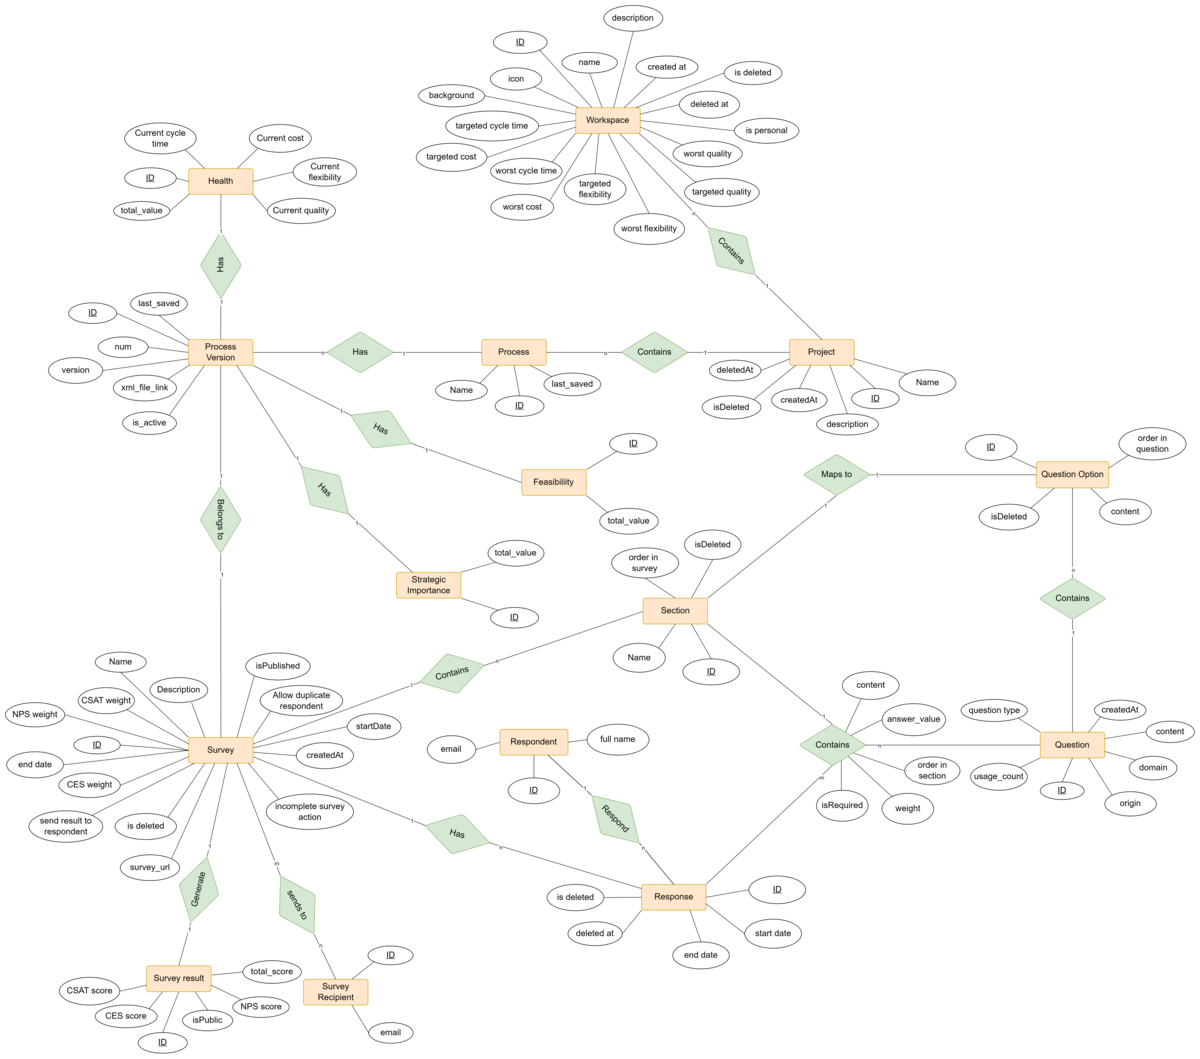
\includegraphics[width=0.8\textwidth]{Content/Phân tích và thiết kế hệ thống/images/erd2-resize.png}
        \vspace{0.5cm}
        \caption{Lược đồ ERD}
        \label{fig:Lược đồ ERD}
\end{figure}

\par
Lược đồ ERD của hệ thống bao gồm các thực thể sau: Workspace, Request,
User, Notification, Project, Process, Process Version, Survey, Survey result, Health, Strategic importance, Feasibility,
Question, Question in survey, Question option, Section, Response, Answer, Respondent, Survey recipient với những
thuộc tính như đã được mô tả ở trên. Các thực thể này có một số
quan hệ như sau, và một số quan hệ cũng có những thuộc tính riêng nó:
\begin{itemize}
    \item Một người dùng có thể tham gia nhiều workspace, một
    workspace có thể có nhiều người dùng tham gia.
    \item Một người dùng có thể tạo nhiều request, một request
    chỉ được tạo bởi một người dùng.
    \item Một workspace có thể quản lý nhiều request, một request
    chỉ thuộc về một workspace.
    \item Một workspace có thể có nhiều project, một project
    chỉ thuộc về một workspace.
    \item Một project có thể có nhiều process, một process
    chỉ thuộc về một project.
    \item Một process có thể có nhiều phiên bản, một phiên bản
    chỉ thuộc về một process.
    \item Một phiên bản process chỉ có thể có một survey.
    \item Một survey có thể có nhiều response, một response chỉ thuộc về một survey.
    \item Một survey chỉ có thể có một survey result.
    \item Một survey có thể có nhiều question, một question chỉ thuộc về một survey.
    \item Một question có thể có nhiều question option, một question option chỉ thuộc về một question.
\end{itemize}

\newpage
\subsection{Ánh xạ ERD và mô tả chi tiết thực thể}

\subsubsection{User: Người dùng của hệ thống}
\begin{center}
        \begin{table}[!h]
        \def\arraystretch{2}
        \resizebox{\textwidth}{!}{
                \begin{tabular}{|p{3cm} |p{2cm} |p{9cm}|}
                        \hline
                        Thuộc tính & Kiểu & Mô tả \\ [0.5ex] 
                        \hline
                        \underline{ID} & integer & ID của người dùng. Khoá chính. \\ 
                        \hline
                        email & varchar & Email của người dùng \\
                        \hline
                        password & varchar & Mật khẩu của người dùng \\
                        \hline
                        phoneNumber & varchar & Số điện thoại của người dùng \\
                        \hline
                        name & text & tên người dùng \\ [1ex] 
                        \hline
                        avatar & text & Đường dẫn tới ảnh đại diện của người dùng \\
                        \hline
                        verified & boolean & True nếu tài khoản đã xác thực, False nếu tài khoản chưa xác thực \\
                        \hline
                \end{tabular}
        }
        \caption{Thực thể User}
        \end{table}
\end{center}
\begin{figure}[H]
        \centering
        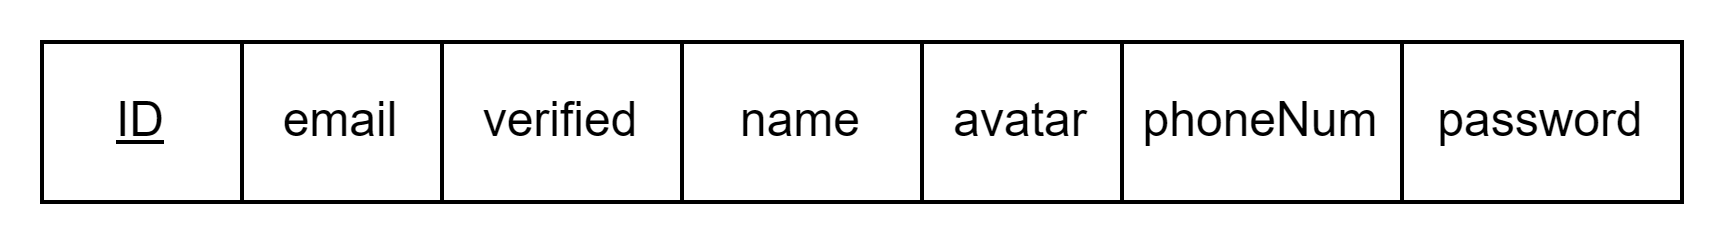
\includegraphics[width=\linewidth]{Content//Phân tích và thiết kế hệ thống//images//ERD_mapping/user_mapping.png}
        \label{fig:Thực thể User}
\end{figure}

\newpage
\subsubsection{Project: Dự án trong workspace}
\begin{center} 
        \begin{table}[H]
                \def\arraystretch{2}%
                \resizebox{\textwidth}{!}{
                        \begin{tabular}{ |p{4cm} |p{3cm} |p{7cm}|} 
                                \hline
                                        Thuộc tính & Kiểu & Mô tả \\ [0.5ex] 
                                \hline
                                        \underline{ID} & integer & ID của project. Khoá chính. \\ 
                                \hline
                                        projectName & text & Tên của project \\
                                \hline
                                        description & text & Mô tả của project \\
                                \hline
                                        isDelete & boolean & Đánh dấu project này đã bị xoá hay chưa \\
                                \hline
                                        createAt & timestamp & Thời gian project được tạo \\
                                \hline
                                        ownerId & integer & ID của người sở hữu project.
                                        Khoá ngoại tham chiếu tới trường Id trong bảng User \\
                                \hline
                                        workspaceId & integer & ID của workspace nơi mà project được tạo. Khoá ngoại tham chiếu tới trường Id trong bảng Workspace \\
                                \hline
                                        deletedAt & timestamp & Thời gian project được xoá khỏi Workspace \\
                                \hline
                                        isWorkspaceDeleted & boolean & Đánh dấu workspace đã bị xoá hay chưa \\
                                \hline
                        \end{tabular}
                }
                \caption{Thực thể Project}
        \end{table}
\end{center}
\begin{figure}[H]
        \centering
        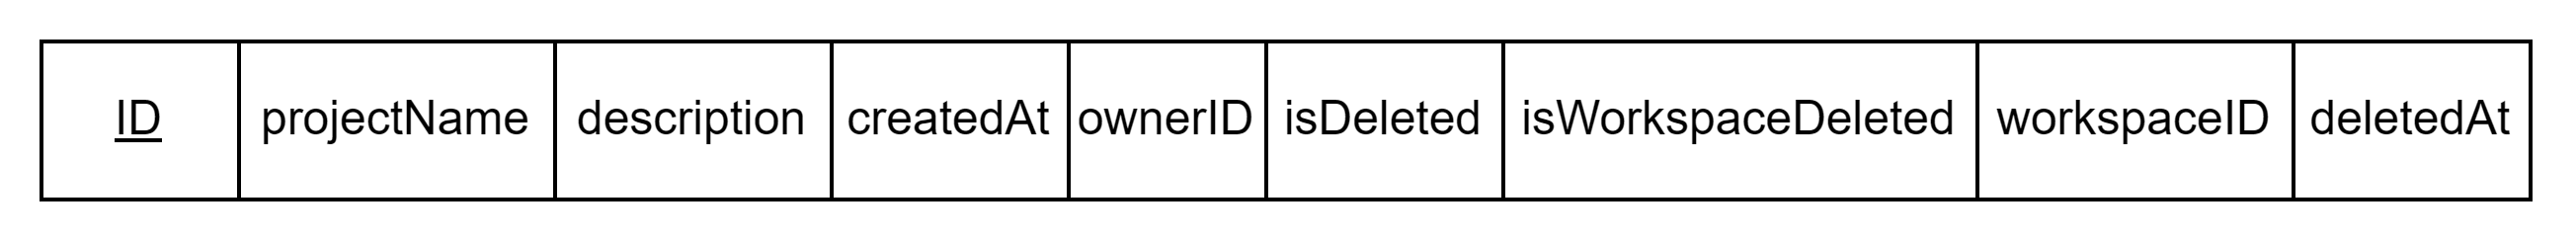
\includegraphics[width=\textwidth]{Content/Phân tích và thiết kế hệ thống/images/ERD_mapping/project_mapping.png}
        \label{fig:Thực thể Project}
\end{figure}

\newpage
\subsubsection{Workspace: Không gian làm việc trong hệ thống}
\begin{center}
        \begin{table}[H]
                \def\arraystretch{2}%
                \resizebox{\textwidth}{!}{
                        \begin{tabular}{ |p{3cm} |p{3cm} |p{8cm}|} 
                                \hline
                                Thuộc tính & Kiểu & Mô tả \\ [0.5ex] 
                                \hline
                                \underline{ID} & integer & ID của workspace. Khoá chính. \\ 
                                \hline
                                name & text & Tên của workspace \\
                                \hline
                                description & text & Mô tả của workspace \\
                                \hline
                                isDeleted & boolean & Đánh dấu workspace đã bị xoá hay chưa \\
                                \hline
                                createAt & timestamp & Thời gian workspace được tạo \\
                                \hline
                                ownerId & integer & ID của người sở hữu workspace.
                                Khoá ngoại tham chiếu tới trường Id trong bảng User \\
                                \hline
                                background & text & Đường link dẫn tới background của workspace \\
                                \hline
                                icon & text & Đường link dẫn tới icon của workspace \\
                                \hline
                                deletedAt & timestamp & Thời gian Workspace được xoá khỏi hệ thống \\
                                \hline
                                isPersonal & boolean & True nếu đây là workspace cá nhân. False nếu là workspace khác \\
                                \hline
                                targeted{\_}cost & double precision & giá trị mục tiêu của độ đo chi phí \\
                                \hline
                                worst{\_}cost & double precision & giá trị tệ nhất của độ đo chi phí \\
                                \hline
                                targeted{\_}cycle{\_}time & double precision & giá trị mục tiêu của độ đo thời gian chu kỳ \\
                                \hline
                                worst{\_}cycle{\_}time & double precision & giá trị tệ nhất của độ đo thời gian chu kỳ \\
                                \hline
                                targeted{\_}quality & double precision & giá trị mục tiêu của độ đo chất lượng \\
                                \hline
                                worst{\_}quality & double precision & giá trị tệ nhất của độ đo chất lượng \\
                                \hline
                                targeted{\_}flexibility & double precision & giá trị mục tiêu của độ đo sự linh hoạt \\
                                \hline
                                worst{\_}flexibility & double precision & giá trị tệ nhất của độ đo sự linh hoạt \\
                                \hline
                        \end{tabular}
                }
                \caption{Thực thể Workspace}
        \end{table}
\end{center}
\begin{figure}[H]
        \centering
        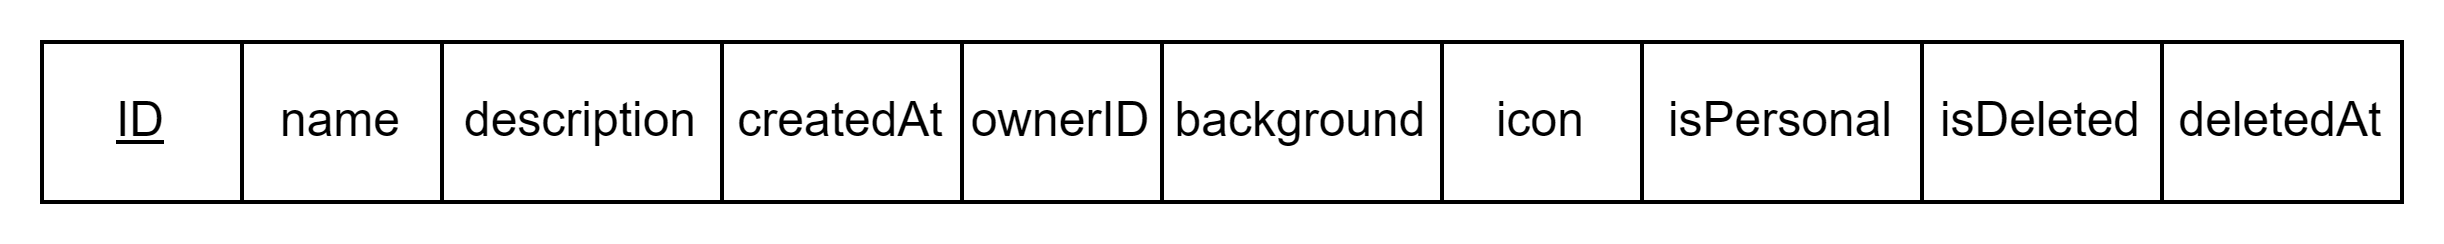
\includegraphics[width=\textwidth]{Content/Phân tích và thiết kế hệ thống/images/ERD_mapping/workspace_mapping.png}
        \label{fig:Thực thể Workspace}
\end{figure}

\newpage
\subsubsection{Join Workspace: Quan hệ tham gia giữa người dùng và workspace}
\begin{center}
        \begin{table}[H]
                \def\arraystretch{2}%
                \resizebox{\textwidth}{!}{
                        \begin{tabular}{ |p{3cm} |p{2cm} |p{9cm} |} 
                                \hline
                                Thuộc tính & Kiểu & Mô tả \\ [0.5ex] 
                                \hline
                                \underline{memberId} & integer & ID của member tham gia Workspace. Khoá ngoại tham chiếu tới trường Id trong User. \\ 
                                \hline
                                \underline{workspaceId} & integer & ID của Workspace. Khoá ngoại tham chiếu tới trường Id trong Workspace. \\
                                \hline
                                joinedAt & timestamp & Thời gian người dùng tham gia Workspace \\
                                \hline
                                isDeleted & boolean & Đánh dấu người dùng đã rời khỏi Workspace hay chưa \\
                                \hline
                                permission & text & Quyền hạn của người dùng khi tham gia Workspace \\
                                \hline
                                leftAt & timestamp & Thời gian người dùng rời khỏi Workspace \\
                                \hline
                                isWorkspaceDeleted & boolean & Đánh dấu workspace đã bị xoá hay chưa \\
                                \hline
                        \end{tabular}
                }
                \caption{Thực thể Join Workspace}
        \end{table}
\end{center}
\begin{figure}[H]
        \centering
        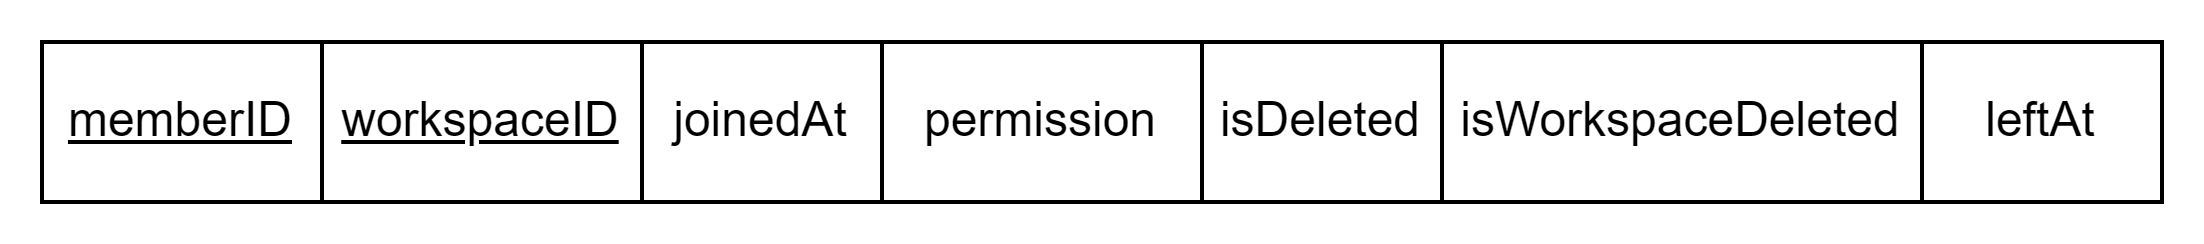
\includegraphics[width=\textwidth]{Content/Phân tích và thiết kế hệ thống/images/ERD_mapping/joinWorkspace_mapping.png}
        \label{fig:Thực thể Join Workspace}
\end{figure}

\subsubsection{Recent Opened Workspace: Quan hệ chỉnh sửa giữa người dùng và workspace}
\begin{center}
        \begin{table}[H]
                \def\arraystretch{2}%
                \resizebox{\textwidth}{!}{
                        \begin{tabular}{ |p{3cm} |p{2cm} |p{9cm}|} 
                                \hline
                                Thuộc tính & Kiểu & Mô tả \\ [0.5ex] 
                                \hline
                                \underline{userId} & integer & ID của member tham gia Workspace. Khoá ngoại tham chiếu tới trường Id trong User. \\ 
                                \hline
                                \underline{workspaceId} & integer & ID của Workspace. Khoá ngoại tham chiếu tới trường Id trong Workspace. \\
                                \hline
                                openedAt & timestamp & Thời gian người dùng mở Workspace lần cuối.\\
                                \hline
                                isHided & boolean & Đánh dấu người dùng đã ẩn Workspace khỏi danh sách của mình hay chưa \\
                                \hline
                                isPinned & boolean & Đánh dấu người dùng đã pin Workspace vào danh sách ưu tiên hay chưa \\
                                \hline
                                isWorkspaceDeleted & boolean & Đánh dấu workspace đã bị xoá hay chưa \\
                                \hline
                        \end{tabular}
                }
                \caption{Thực thể Recent Opened Workspace}
        \end{table}  
\end{center}
\begin{figure}[H]
        \centering
        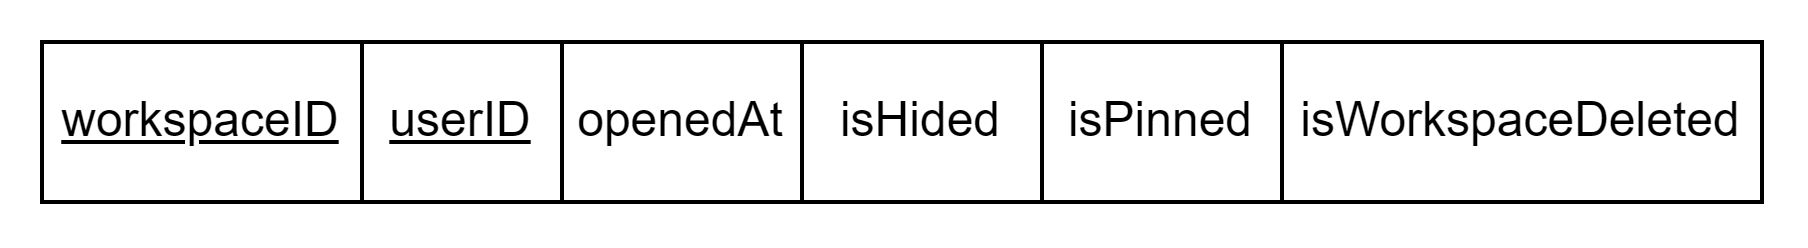
\includegraphics[width=\textwidth]{Content/Phân tích và thiết kế hệ thống/images/ERD_mapping/recent_opened_workspace_mapping.png}
        \label{fig:Thực thể Recent Opened Workspace}
\end{figure}

\subsubsection{Request: Các yêu cầu trong hệ thống}
\begin{center}
        \begin{table}[H]
                \def\arraystretch{2}%
                \resizebox{\textwidth}{!}{
                        \begin{tabular}{ |p{3cm} |p{3cm} |p{9cm}|} 
                                \hline
                                Thuộc tính & Kiểu & Mô tả \\ [0.5ex] 
                                \hline
                                \underline{ID} & integer & ID của request. Khoá chính \\ 
                                \hline
                                type & varchar & Kiểu request \\
                                \hline
                                createdAt & timestamp & Thời gian người dùng tạo request.\\
                                \hline
                                status & text & Trạng thái của request, đang được xử lý hay đã được chấp thuận, từ chối.\\
                                \hline
                                isDeleted & boolean & Đánh dấu request bị xoá hay chưa \\
                                \hline
                                isWorkspaceDeleted & boolean & Đánh dấu workspace đã bị xoá hay chưa \\
                                \hline
                                workspaceId & integer & ID của workspace chứa request đó. Khoá ngoại tham chiếu tới trường Id trong Workspace \\
                                \hline
                                senderId & integer & ID của người gửi request. Khoá ngoại tham chiếu tới trường Id trong User \\
                                \hline
                                recipientId & integer & ID của người nhận request đã xử lý. Khoá ngoại tham chiếu tới trường Id trong User \\
                                \hline
                                handlerId & integer & ID của người xử lý request. Khoá ngoại tham chiếu tới trường Id trong User \\
                                \hline
                                frPermission & text & permission hiện tại của người gửi. \\
                                \hline
                                toPermission & text & permission mong muốn của người gửi. \\
                                \hline
                                rcpPermission & text & permission của người sẽ nhận được lời mời tham gia workspace. \\
                                \hline
                                deletedAt & timestamp & Thời gian xoá request. \\
                                \hline
                        \end{tabular}
                }
                \caption{Thực thể Request}
        \end{table}
\end{center}
\begin{figure}[H]
        \centering
        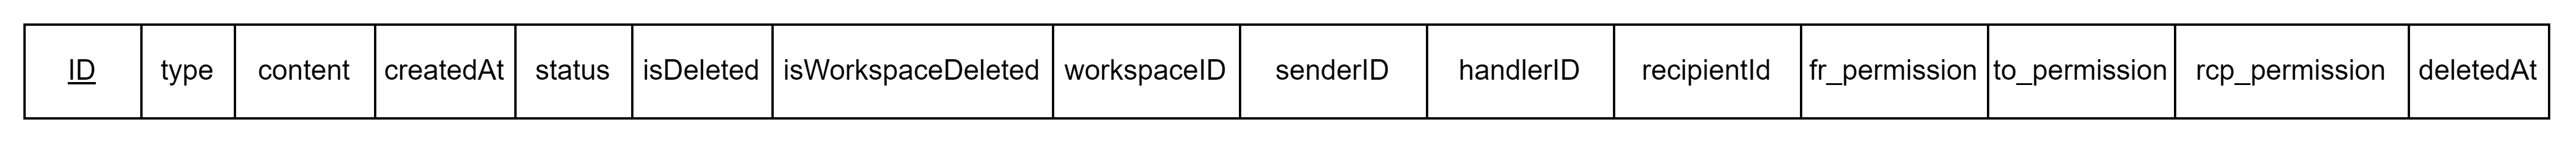
\includegraphics[width=\textwidth]{Content/Phân tích và thiết kế hệ thống/images/ERD_mapping/request_mapping.png}
        \label{fig:Thực thể request}
\end{figure}

\subsubsection{Notification: Các thông báo của người dùng}
\begin{center}
        \begin{table}[H]
                \def\arraystretch{2}%
                \resizebox{\textwidth}{!}{
                \begin{tabular}{ |p{3cm} |p{3cm} |p{9cm}|} 
                        \hline
                           Thuộc tính & Kiểu & Mô tả \\ [0.5ex] 
                        \hline
                        \underline{ID} & integer & ID của thông báo. Khoá chính \\ 
                        \hline
                        notificationType & varchar & Kiểu thông báo \\
                        \hline
                        createdAt & timestamp & Thời gian người dùng nhận được thông báo.\\
                        \hline
                        status & text & Trạng thái của thông báo, đã được chấp thuận hay đồng ý hoặc từ chối lời mời.\\
                        \hline
                        isDeleted & boolean & Đánh dấu thông báo bị xoá hay chưa \\
                        \hline
                        isStarred & boolean & Đánh dấu thông báo đã được đánh dấu ưu tiên hay chưa \\
                        \hline
                        workspaceId & integer & ID của workspace gửi thông báo đó. Khoá ngoại tham chiếu tới trường Id trong Workspace \\
                        \hline
                         isRead & boolean & Đánh dấu thông báo đã được đọc hay chưa \\
                        \hline
                         permission & text & permission của người nhận. \\
                        \hline
                         deletedAt & timestamp & Thời gian xoá request. \\
                        \hline
                \end{tabular}}
                \caption{Thực thể Notification}
        \end{table}
\end{center}
\begin{figure}[H]
        \centering
        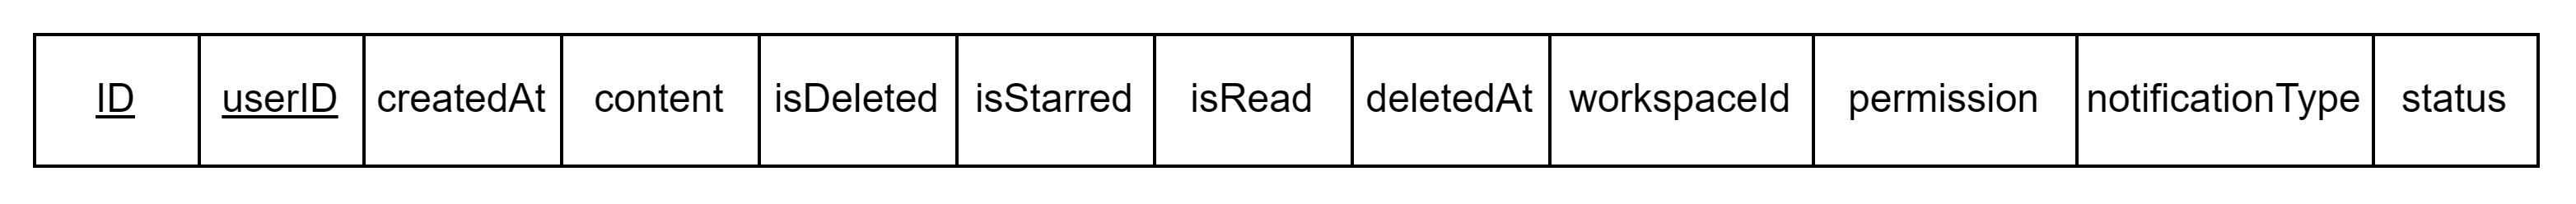
\includegraphics[width=\textwidth]{Content/Phân tích và thiết kế hệ thống/images/ERD_mapping/notification_mapping.png}
        \label{fig:Thực thể Notification}
\end{figure}

\subsubsection{Process version: Phiên bản của quy trình}
\begin{center}
        \begin{table}[H]
                \def\arraystretch{2}%
                \resizebox{\textwidth}{!}{
                \begin{tabular}{ |p{3cm} |p{3cm} |p{9cm}|} 
                        \hline
                        Thuộc tính & Kiểu & Mô tả \\ [0.5ex] 
                        \hline
                        \underline{ID} & integer & ID của phiên bản quy trình. Khoá chính \\ 
                        \hline
                        version & integer & Số phiên bản của quy trình \\
                        \hline
                        xml{\_}file{\_}link & varchar & Đường dẫn link tới file BPMN.\\
                        \hline
                        isDeleted & boolean & Đánh dấu phiên bản quy trình bị xoá hay chưa \\
                        \hline
                        process{\_}id & integer & ID của quy trình. Khoá ngoại tham chiếu tới trường Id trong Process \\
                        \hline
                        project{\_}id & integer & ID của project. Khoá ngoại tham chiếu tới trường Id trong Project \\
                        \hline
                        deleted{\_}at & timestamp & Thời gian xoá phiên bản quy trình. \\
                        \hline
                        last{\_}saved & timestamp & Thời gian lưu phiên bản quy trình cuối cùng. \\
                        \hline
                        is{\_}active & boolean & Đánh dấu phiên bản quy trình đang hoạt động hay không. \\
                        \hline
                \end{tabular}}
                \caption{Thực thể Process Version}
        \end{table}
\end{center}
\begin{figure}[H]
        \centering
        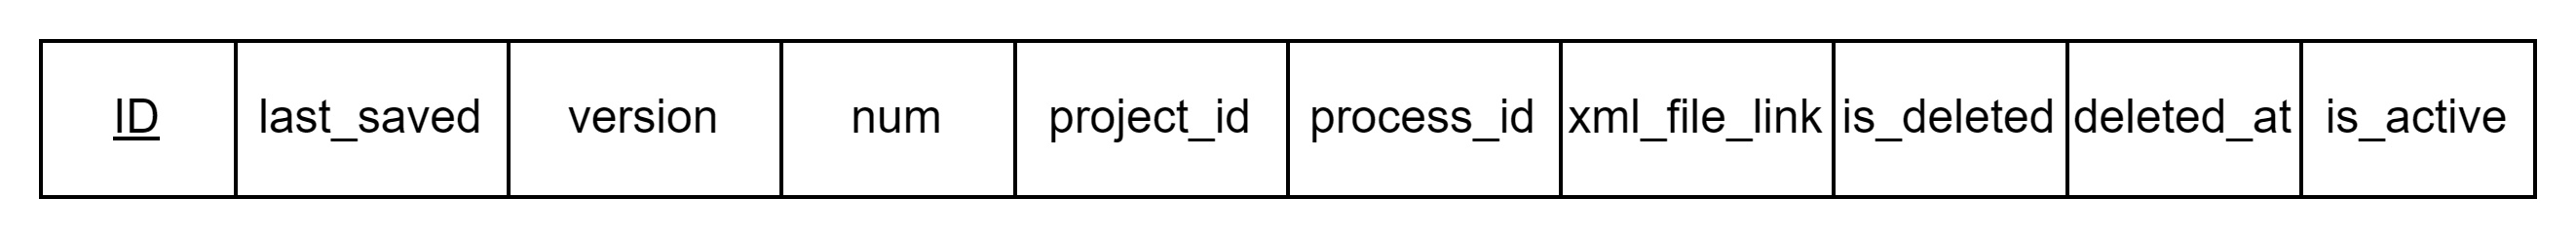
\includegraphics[width=\textwidth]{Content/Phân tích và thiết kế hệ thống/images/ERD_mapping/process_version_mapping.png}
        \label{fig:Thực thể Process Version}
\end{figure}

\subsubsection{Survey: Bài khảo sát}
\begin{center}
        \begin{table}[H]
                \def\arraystretch{2}%
                \resizebox{\textwidth}{!}{
                        \begin{tabular}{ |p{4.5cm} |p{3cm} |p{6.5cm}|} 
                                \hline
                                Thuộc tính & Kiểu & Mô tả \\ [0.5ex] 
                                \hline
                                \underline{ID} & integer & ID của bài khảo sát. Khoá chính \\ 
                                \hline
                                name & text & Tên của bài khảo sát \\
                                \hline
                                description & text & Mô tả của bài khảo sát \\
                                \hline
                                is{\_}deleted & boolean & Đánh dấu bài khảo sát bị xoá hay chưa \\
                                \hline
                                created{\_}at & timestamp & Thời gian bài khảo sát được tạo \\
                                \hline
                                start{\_}date & timestamp & Thời gian bài khảo sát được publish \\
                                \hline
                                process{\_}version{\_}version & varchar & phiên bản của process chứa bài khảo sát. Khoá ngoại tham chiếu tới trường version trong Process version \\
                                \hline
                                deleted{\_}at & timestamp & Thời gian bài khảo sát được xoá khỏi hệ thống \\
                                \hline
                                is{\_}published & boolean & Đánh dấu bài khảo sát đã được publish hay chưa \\
                                \hline
                                end{\_}date & timestamp & Thời gian kết thúc bài khảo sát \\
                                \hline
                                allow{\_}duplicate{\_}respondent & boolean & Cho phép người dùng trả lời bài khảo sát nhiều lần hay không \\
                                \hline
                                send{\_}result{\_}to{\_}respondent & boolean & Gửi kết quả khảo sát cho người trả lời hay không \\
                                \hline
                                survey{\_}url & varchar & Đường dẫn tới bài khảo sát \\
                                \hline
                                ces{\_}weight & double precision & Trọng số của độ đo CES \\
                                \hline
                                nps{\_}weight & double precision & Trọng số của độ đo NPS \\
                                \hline
                                csat{\_}weight & double precision & Trọng số của độ đo CSAT \\
                                \hline
                                domain & varchar & Lĩnh vực của bài khảo sát \\
                                \hline
                                last{\_}saved & timestamp & Thời gian lưu bài khảo sát cuối cùng \\
                                \hline
                                incomplete{\_}response{\_}action & varchar & Hành động đối với những bài khảo sát đang làm dở của người dùng \\
                        \end{tabular}
                }
                \caption{Thực thể Survey}
        \end{table}
\end{center}
\begin{figure}[H]
        \centering
        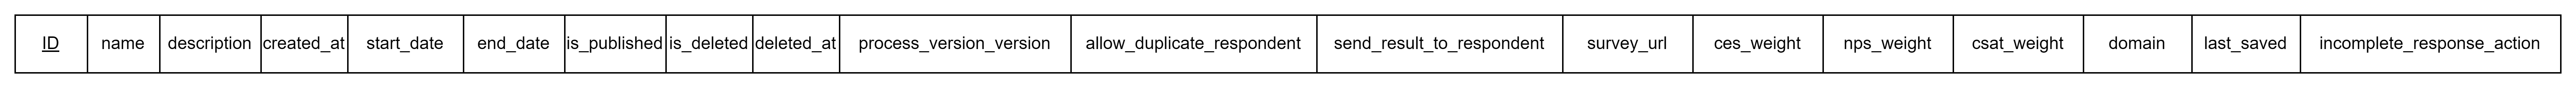
\includegraphics[width=\textwidth]{Content/Phân tích và thiết kế hệ thống/images/ERD_mapping/survey_mapping.png}
        \label{fig:Thực thể Survey}
\end{figure}

\subsubsection{Health: Sức khoẻ của quy trình}
\begin{center}
        \begin{table}[H]
                \def\arraystretch{2}%
                \resizebox{\textwidth}{!}{
                        \begin{tabular}{ |p{4cm} |p{3cm} |p{7cm}|} 
                                \hline
                                Thuộc tính & Kiểu & Mô tả \\ [0.5ex] 
                                \hline
                                \underline{ID} & integer & ID của sức khoẻ. Khoá chính \\ 
                                \hline
                                process{\_}version{\_}version & integer & phiên bản của process chứa sức khoẻ. Khoá ngoại tham chiếu tới trường version trong Process version \\
                                \hline
                                current{\_}cycle{\_}time & double precision & Giá trị hiện tại của độ đo thời gian \\
                                \hline
                                current{\_}cost & double precision & Giá trị hiện tại của độ đo chi phí \\
                                \hline
                                current{\_}quality & double precision & Giá trị hiện tại của độ đo chất lượng \\
                                \hline
                                current{\_}flexibility & double precision & Giá trị hiện tại của độ đo sự linh hoạt \\
                                \hline
                        \end{tabular}
                }
                \caption{Thực thể Health}
        \end{table}
\end{center}
\begin{figure}[H]
        \centering
        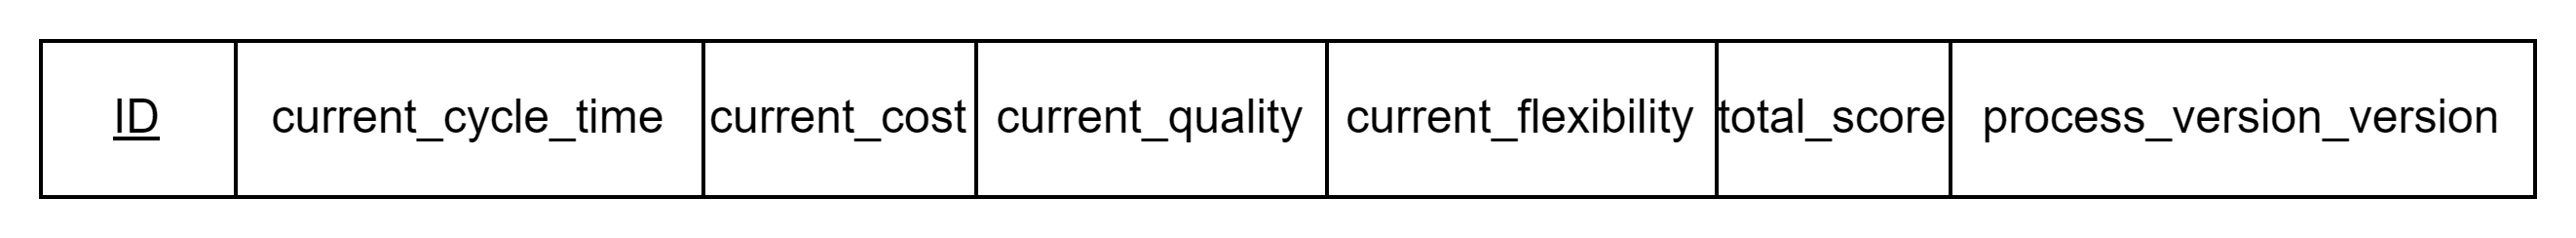
\includegraphics[width=\textwidth]{Content/Phân tích và thiết kế hệ thống/images/ERD_mapping/health_mapping.png}
        \label{fig:Thực thể Health}
\end{figure}

\subsubsection{Strategic Importance: Mức độ quan trọng chiến lược của quy trình}
\begin{center}
        \begin{table}[H]
                \def\arraystretch{2}%
                \resizebox{\textwidth}{!}{
                        \begin{tabular}{ |p{4cm} |p{3cm} |p{7cm}|} 
                                \hline
                                Thuộc tính & Kiểu & Mô tả \\ [0.5ex] 
                                \hline
                                \underline{ID} & integer & ID của mức độ quan trọng chiến lược. Khoá chính \\ 
                                \hline
                                process{\_}version{\_}version & integer & phiên bản của process chứa mức độ quan trọng chiến lược. Khoá ngoại tham chiếu tới trường version trong Process version \\
                                \hline
                                total{\_}value & double precision & Giá trị mức độ quan trọng chiến lược \\
                                \hline
                        \end{tabular}
                }
                \caption{Thực thể Strategic Importance}
        \end{table}
\end{center}
\begin{figure}[H]
        \centering
        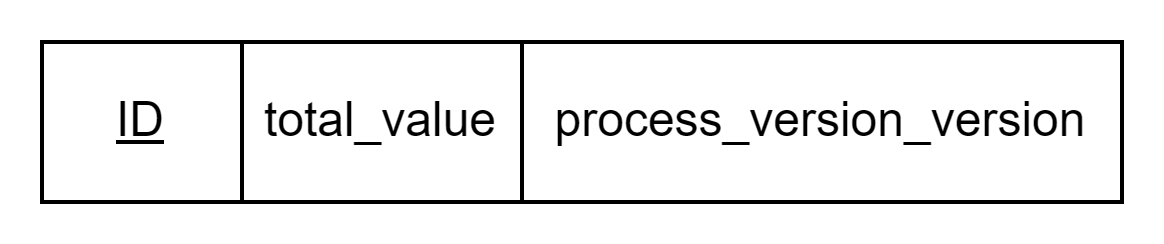
\includegraphics[width=0.5\textwidth]{Content/Phân tích và thiết kế hệ thống/images/ERD_mapping/strategic_importance_mapping.png}
        \label{fig:Thực thể Strategic Importance}
\end{figure}

\subsubsection{Feasibility: Mức độ khả thi của quy trình}
\begin{center}
        \begin{table}[H]
                \def\arraystretch{2}%
                \resizebox{\textwidth}{!}{
                        \begin{tabular}{ |p{4cm} |p{3cm} |p{7cm}|} 
                                \hline
                                Thuộc tính & Kiểu & Mô tả \\ [0.5ex] 
                                \hline
                                \underline{ID} & integer & ID của mức độ khả thi. Khoá chính \\ 
                                \hline
                                process{\_}version{\_}version & integer & phiên bản của process chứa mức độ khả thi. Khoá ngoại tham chiếu tới trường version trong Process version \\
                                \hline
                                total{\_}value & double precision & Giá trị mức độ khả thi \\
                                \hline
                        \end{tabular}
                }
                \caption{Thực thể Feasibility}
        \end{table}
\end{center}
\begin{figure}[H]
        \centering
        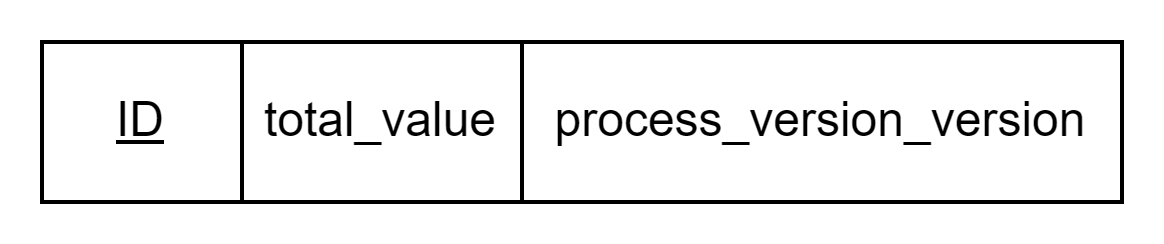
\includegraphics[width=0.5\textwidth]{Content/Phân tích và thiết kế hệ thống/images/ERD_mapping/feasibility_mapping.png}
        \label{fig:Thực thể Feasibility}
\end{figure}

\subsubsection{Survey result: Kết quả khảo sát}
\begin{center}
        \begin{table}[H]
                \def\arraystretch{2}%
                \resizebox{\textwidth}{!}{
                        \begin{tabular}{ |p{3cm} |p{3cm} |p{9cm}|} 
                                \hline
                                Thuộc tính & Kiểu & Mô tả \\ [0.5ex] 
                                \hline
                                \underline{ID} & integer & ID của kết quả khảo sát. Khoá chính \\ 
                                \hline
                                survey{\_}id & integer & ID của bài khảo sát. Khoá ngoại tham chiếu tới trường ID trong Survey \\
                                \hline
                                ces{\_}score & double precision & Giá trị độ đo CES \\
                                \hline
                                nps{\_}score & double precision & Giá trị độ đo NPS \\
                                \hline
                                csat{\_}score & double precision & Giá trị độ đo CSAT \\
                                \hline
                                total{\_}score & double precision & Giá trị tổng của bài khảo sát \\
                                \hline
                                visibility & boolean & Đánh dấu kết quả survey có thể xem bởi những người dùng khác ngoài project owner không
                                \\
                                \hline
                        \end{tabular}
                }
                \caption{Thực thể Survey Result}
        \end{table}
\end{center}
\begin{figure}[H]
        \centering
        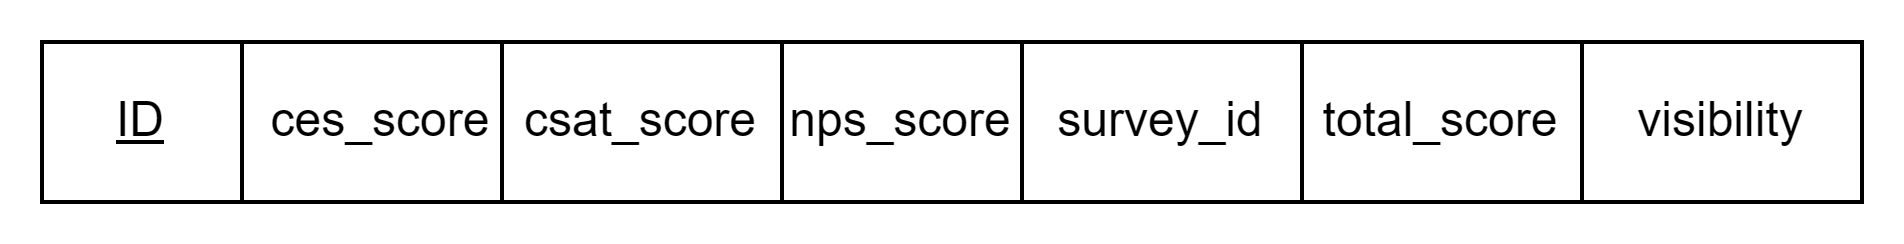
\includegraphics[width=\textwidth]{Content/Phân tích và thiết kế hệ thống/images/ERD_mapping/survey_result_mapping.png}
        \label{fig:Thực thể Survey Result}
\end{figure}

\subsubsection{Response: Phản hồi của người dùng}
\begin{center}
        \begin{table}[H]
                \def\arraystretch{2}%
                \resizebox{\textwidth}{!}{
                        \begin{tabular}{ |p{3cm} |p{3cm} |p{9cm}|} 
                                \hline
                                Thuộc tính & Kiểu & Mô tả \\ [0.5ex] 
                                \hline
                                \underline{ID} & integer & ID của phản hồi. Khoá chính \\ 
                                \hline
                                survey{\_}id & integer & ID của bài khảo sát. Khoá ngoại tham chiếu tới trường ID trong Survey \\
                                \hline
                                respondent{\_}id & integer & ID của người trả lời. Khoá ngoại tham chiếu tới trường ID trong Respondent \\
                                \hline
                                start{\_}date & timestamp & Thời điểm người dùng thực hiện bài làm khảo sát \\
                                \hline
                                end{\_}date & timestamp & Thời điểm người dùng submit bài làm khảo sát \\
                                \hline
                                is{\_}deleted & boolean & Đánh dấu phản hồi bị xoá hay chưa \\
                                \hline
                        \end{tabular}
                }
                \caption{Thực thể Response}
        \end{table}
\end{center}
\begin{figure}[H]
        \centering
        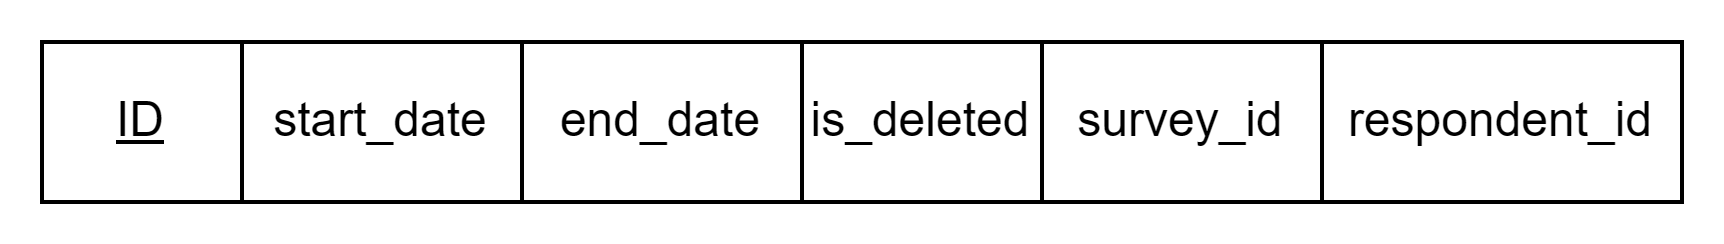
\includegraphics[width=\textwidth]{Content/Phân tích và thiết kế hệ thống/images/ERD_mapping/response_mapping.png}
        \label{fig:Thực thể Response}
\end{figure}

\subsubsection{Respondent: Người trả lời khảo sát}
\begin{center}
        \begin{table}[H]
                \def\arraystretch{2}%
                \resizebox{\textwidth}{!}{
                        \begin{tabular}{ |p{3cm} |p{3cm} |p{9cm}|} 
                                \hline
                                Thuộc tính & Kiểu & Mô tả \\ [0.5ex] 
                                \hline
                                \underline{ID} & integer & ID của người trả lời. Khoá chính \\ 
                                \hline
                                email & varchar & Email của người trả lời \\
                                \hline
                                full{\_}name & text & Tên của người trả lời \\
                                \hline
                        \end{tabular}
                }
                \caption{Thực thể Respondent}
        \end{table}
\end{center}
\begin{figure}[H]
        \centering
        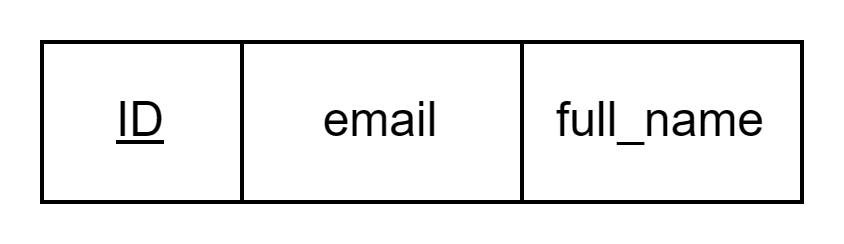
\includegraphics[width=0.5\textwidth]{Content/Phân tích và thiết kế hệ thống/images/ERD_mapping/respondent_mapping.png}
        \label{fig:Thực thể Respondent}
\end{figure}

\subsubsection{Answer: Câu trả lời của người dùng trong khảo sát}
\begin{center}
        \begin{table}[H]
                \def\arraystretch{2}%
                \resizebox{\textwidth}{!}{
                        \begin{tabular}{ |p{3cm} |p{3cm} |p{9cm}|} 
                                \hline
                                Thuộc tính & Kiểu & Mô tả \\ [0.5ex] 
                                \hline
                                \underline{ID} & integer & ID của câu trả lời. Khoá chính \\ 
                                \hline
                                response{\_}id & integer & ID của phản hồi. Khoá ngoại tham chiếu tới trường ID trong Response \\
                                \hline
                                question{\_}id & integer & ID của câu hỏi. Khoá ngoại tham chiếu tới trường ID trong Question \\
                                \hline
                                value & varchar & Câu trả lời của người dùng \\
                                \hline
                        \end{tabular}
                }
                \caption{Thực thể Answer}
        \end{table}
\end{center}
\begin{figure}[H]
        \centering
        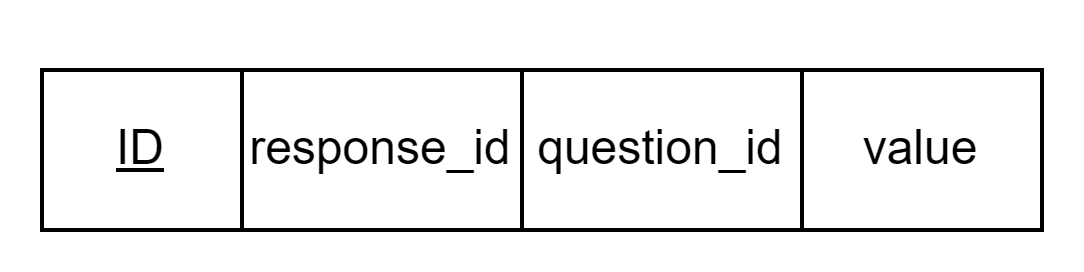
\includegraphics[width=0.5\textwidth]{Content/Phân tích và thiết kế hệ thống/images/ERD_mapping/answer_mapping.png}
        \label{fig:Thực thể Answer}
\end{figure}

\subsubsection{Question in section: Câu hỏi trong một phần của khảo sát}
\begin{center}
        \begin{table}[H]
                \def\arraystretch{2}%
                \resizebox{\textwidth}{!}{
                        \begin{tabular}{ |p{3cm} |p{3cm} |p{9cm}|} 
                                \hline
                                Thuộc tính & Kiểu & Mô tả \\ [0.5ex] 
                                \hline
                                \underline{ID} & integer & ID của câu hỏi. Khoá chính \\ 
                                \hline
                                content & varchar & Nội dung của câu hỏi \\
                                \hline
                                section{\_}id & integer & ID của phần. Khoá ngoại tham chiếu tới trường ID trong Section \\
                                \hline
                                question{\_}id & integer & ID của câu hỏi. Khoá ngoại tham chiếu tới trường ID trong Question \\
                                \hline
                                order{\_}in{\_}section & integer & Thứ tự của câu hỏi trong phần \\
                                \hline
                                weight & double precision & Trọng số của câu hỏi \\
                                \hline
                                is{\_}required & boolean & Đánh dấu câu hỏi có bắt buộc hay không \\
                                \hline
                                question{\_}type & varchar & Loại câu hỏi \\
                                \hline
                        \end{tabular}
                }
                \caption{Thực thể Question in section}
        \end{table}
\end{center}
\begin{figure}[H]
        \centering
        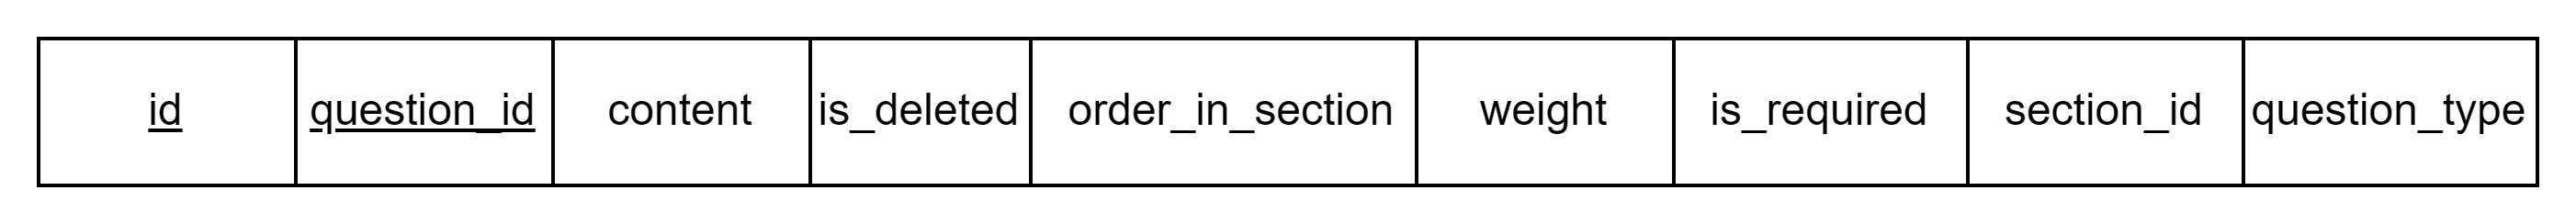
\includegraphics[width=\textwidth]{Content/Phân tích và thiết kế hệ thống/images/ERD_mapping/question_in_section_mapping.png}
        \label{fig:Thực thể Question in section}
\end{figure}

\subsubsection{Section in survey: Phần của khảo sát}
\begin{center}
        \begin{table}[H]
                \def\arraystretch{2}%
                \resizebox{\textwidth}{!}{
                        \begin{tabular}{ |p{3cm} |p{3cm} |p{9cm}|} 
                                \hline
                                Thuộc tính & Kiểu & Mô tả \\ [0.5ex] 
                                \hline
                                \underline{ID} & integer & ID của phần. Khoá chính \\ 
                                \hline
                                name & varchar & Tên của phần \\
                                \hline
                                survey{\_}id & integer & ID của bài khảo sát. Khoá ngoại tham chiếu tới trường ID trong Survey \\
                                \hline
                                order{\_}in{\_}survey & integer & Thứ tự của phần trong bài khảo sát \\
                                \hline
                                is{\_}deleted & boolean & Đánh dấu phần bị xoá hay chưa \\
                                \hline
                        \end{tabular}
                }
                \caption{Thực thể Section in survey}
        \end{table}
\end{center}
\begin{figure}[H]
        \centering
        
\includegraphics[width=\textwidth]{Content/Phân tích và thiết kế hệ thống/images/ERD_mapping/section_in_survey_mapping.png}
        \label{fig:Thực thể Section in survey}
\end{figure}

\subsubsection{Question option: Câu trả lời của câu hỏi trong khảo sát}
\begin{center}
        \begin{table}[H]
                \def\arraystretch{2}%
                \resizebox{\textwidth}{!}{
                        \begin{tabular}{ |p{3cm} |p{3cm} |p{9cm}|} 
                                \hline
                                Thuộc tính & Kiểu & Mô tả \\ [0.5ex] 
                                \hline
                                \underline{ID} & integer & ID của câu trả lời. Khoá chính \\ 
                                \hline
                                question{\_}id & integer & ID của câu hỏi. Khoá ngoại tham chiếu tới trường ID trong Question \\
                                \hline
                                value & varchar & Nội dung của câu trả lời \\
                                \hline
                                is{\_}deleted & boolean & Đánh dấu câu trả lời bị xoá hay không \\
                                \hline
                                question{\_}in{\_}section{\_}id & integer & ID của câu hỏi trong phần. Khoá ngoại tham chiếu tới trường ID trong Question in section \\
                                \hline
                                order & integer & Thứ tự của câu trả lời trong câu hỏi \\
                                \hline
                        \end{tabular}}
                \caption{Thực thể Question option}
        \end{table}
\end{center}
\begin{figure}[H]
        \centering
        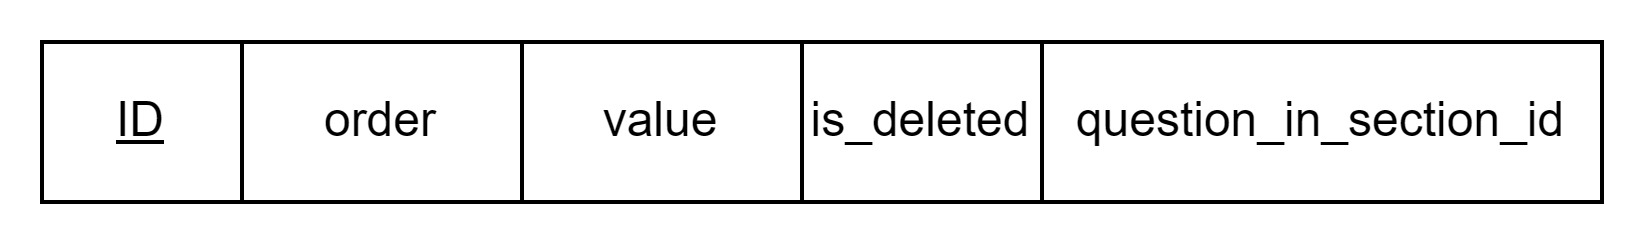
\includegraphics[width=\textwidth]{Content/Phân tích và thiết kế hệ thống/images/ERD_mapping/question_option_mapping.png}
        \label{fig:Thực thể Question option}
\end{figure}

\subsubsection{Question option Section mapping: Liên kết giữa câu hỏi và phần của khảo sát với câu trả lời của câu hỏi đó}
\begin{center}
        \begin{table}[H]
                \def\arraystretch{2}%
                \resizebox{\textwidth}{!}{
                \begin{tabular}{ |p{3cm} |p{3cm} |p{9cm}|} 
                        \hline
                        Thuộc tính & Kiểu & Mô tả \\ [0.5ex] 
                        \hline
                        \underline{section{\_}id} & integer & ID của phần trong khảo sát. Khoá ngoại tham chiếu tới trường ID trong Section \\
                        \hline
                        \underline{question{\_}option{\_}id} & integer & ID của câu trả lời. Khoá ngoại tham chiếu tới trường ID trong Question option \\
                        \hline
                        is{\_}deleted & boolean & Đánh dấu liên kết bị xoá hay không \\ 
                        \hline
                \end{tabular}}
                \caption{Thực thể Question option Section mapping}
        \end{table}
\end{center}
\begin{figure}[H]
        \centering
        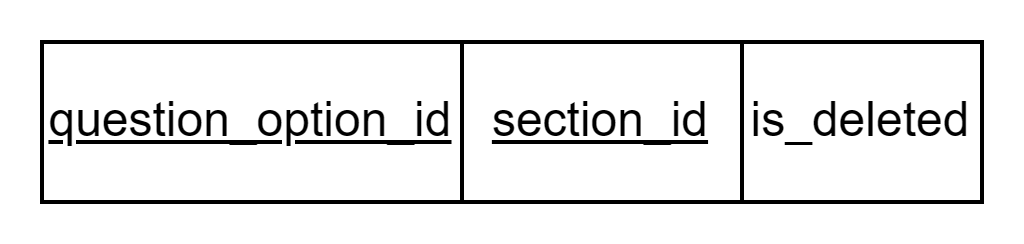
\includegraphics[width=0.5\textwidth]{Content/Phân tích và thiết kế hệ thống/images/ERD_mapping/question_option_section_mapping.png}
        \label{fig:Thực thể Question option Section mapping}
\end{figure}

\subsubsection{Question: Câu hỏi trong hệ thống}
\begin{center}
        \begin{table}[H]
                \def\arraystretch{2}%
                \resizebox{\textwidth}{!}{
                \begin{tabular}{ |p{3cm} |p{3cm} |p{9cm}|} 
                        \hline
                        Thuộc tính & Kiểu & Mô tả \\ [0.5ex] 
                        \hline
                        \underline{ID} & integer & ID của câu hỏi. Khoá chính \\ 
                        \hline
                        content & varchar & Nội dung của câu hỏi \\
                        \hline
                        is{\_}deleted & boolean & Đánh dấu câu hỏi bị xoá hay không \\
                        \hline
                        question{\_}type & varchar & Loại câu hỏi \\
                        \hline
                        created{\_}at & timestamp & Thời gian câu hỏi được tạo \\
                        \hline
                        origin & varchar & Nguồn của câu hỏi \\
                        \hline
                        domain & varchar & Lĩnh vực của câu hỏi \\
                        \hline
                        contributor{\_}id & integer & ID của người đóng góp câu hỏi. Khoá ngoại tham chiếu tới trường ID trong User \\
                        \hline
                        usage{\_}count & integer & Số lần câu hỏi được sử dụng \\
                        \hline
                \end{tabular}}
                \caption{Thực thể Question}
        \end{table}
\end{center}
\begin{figure}[H]
        \centering
        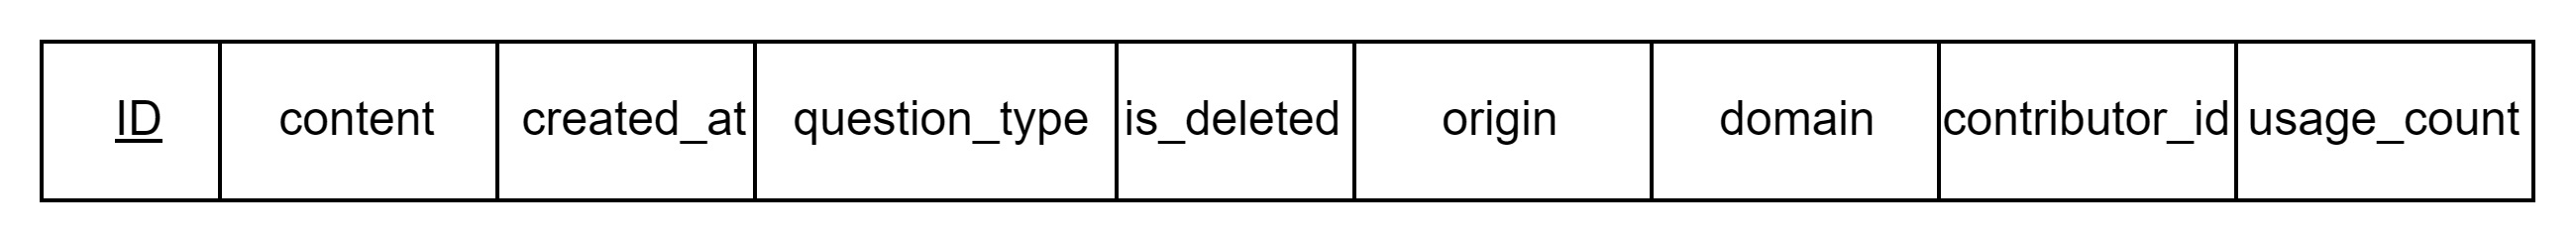
\includegraphics[width=\textwidth]{Content/Phân tích và thiết kế hệ thống/images/ERD_mapping/question_mapping.png}
        \label{fig:Thực thể Question}
\end{figure}

\subsubsection{Survey recipient: Người nhận khảo sát}
\begin{center}
        \begin{table}[H]
                \def\arraystretch{2}%
                \resizebox{\textwidth}{!}{
                \begin{tabular}{ |p{3cm} |p{3cm} |p{9cm}|} 
                        \hline
                        Thuộc tính & Kiểu & Mô tả \\ [0.5ex] 
                        \hline
                        \underline{ID} & integer & ID của người nhận khảo sát. Khoá chính \\ 
                        \hline
                        email & varchar & Email của người nhận \\
                        \hline
                \end{tabular}}
                \caption{Thực thể Survey Recipient}
        \end{table}
\end{center}
\begin{figure}[H]
        \centering
        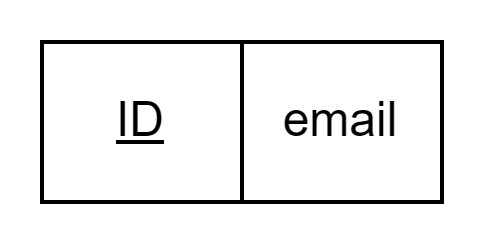
\includegraphics[width=0.25\textwidth]{Content/Phân tích và thiết kế hệ thống/images/ERD_mapping/survey_recipient_mapping.png}
        \label{fig:Thực thể Survey Recipient}
\end{figure}

\subsubsection{Send survey: Gửi khảo sát cho người nhận khảo sát}
\begin{center}
        \begin{table}[H]
                \def\arraystretch{2}%
                \resizebox{\textwidth}{!}{
                \begin{tabular}{ |p{3cm} |p{3cm} |p{9cm}|} 
                        \hline
                        Thuộc tính & Kiểu & Mô tả \\ [0.5ex] 
                        \hline
                        \underline{survey{\_}id} & integer & ID của bài khảo sát. Khoá ngoại tham chiếu tới trường ID trong Survey \\
                        \hline
                        \underline{recipient{\_}id} & integer & ID của người nhận khảo sát. Khoá ngoại tham chiếu tới trường ID trong Survey Recipient \\
                        \hline
                \end{tabular}}
                \caption{Thực thể Send Survey}
        \end{table}
\end{center}
\begin{figure}[H]
        \centering
        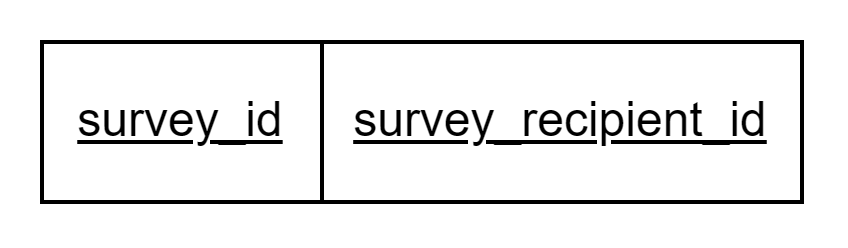
\includegraphics[width=0.5\textwidth]{Content/Phân tích và thiết kế hệ thống/images/ERD_mapping/send_survey_mapping.png}
        \label{fig:Thực thể Send Survey}
\end{figure}